\chapter{Evaluation}
%
\section{Boost Converter}
The characteristic curve of the boost converter is examined. In \vref{fig:characteristic-curve-of-the-boost-converter} the output voltage is plotted against the duty cycle.
\begin{figure}[H]
  \centering
  \includegraphics[width=1\linewidth]{messdaten/Characteristic Curve of the Boost Converter}
  \caption[characteristic curve of the boost converter]{characteristic curve of the boost converter}
  \label{fig:characteristic-curve-of-the-boost-converter}
\end{figure}
SciDAVis returns the linear fit of the measuring points as
\begin{equation}
U_{out}(dc)=\SI{1.51}{\frac{V}{\%}} \cdot dc + \SI{9.07}{V}
\end{equation}
If the output voltages are compared with the simulated ones, there is observed a deviation of nearly \SI{10}{V} in the higher voltage area. The lower voltages, however, are similar.

\section{Avalanche Pulse Generator}
The signal in \vref{fig:img20201201084956} is the first that appears after increasing the voltage to the minimum voltage $ U_{min}=\SI{70}{V} $.
\begin{figure}[H]
 \centering
 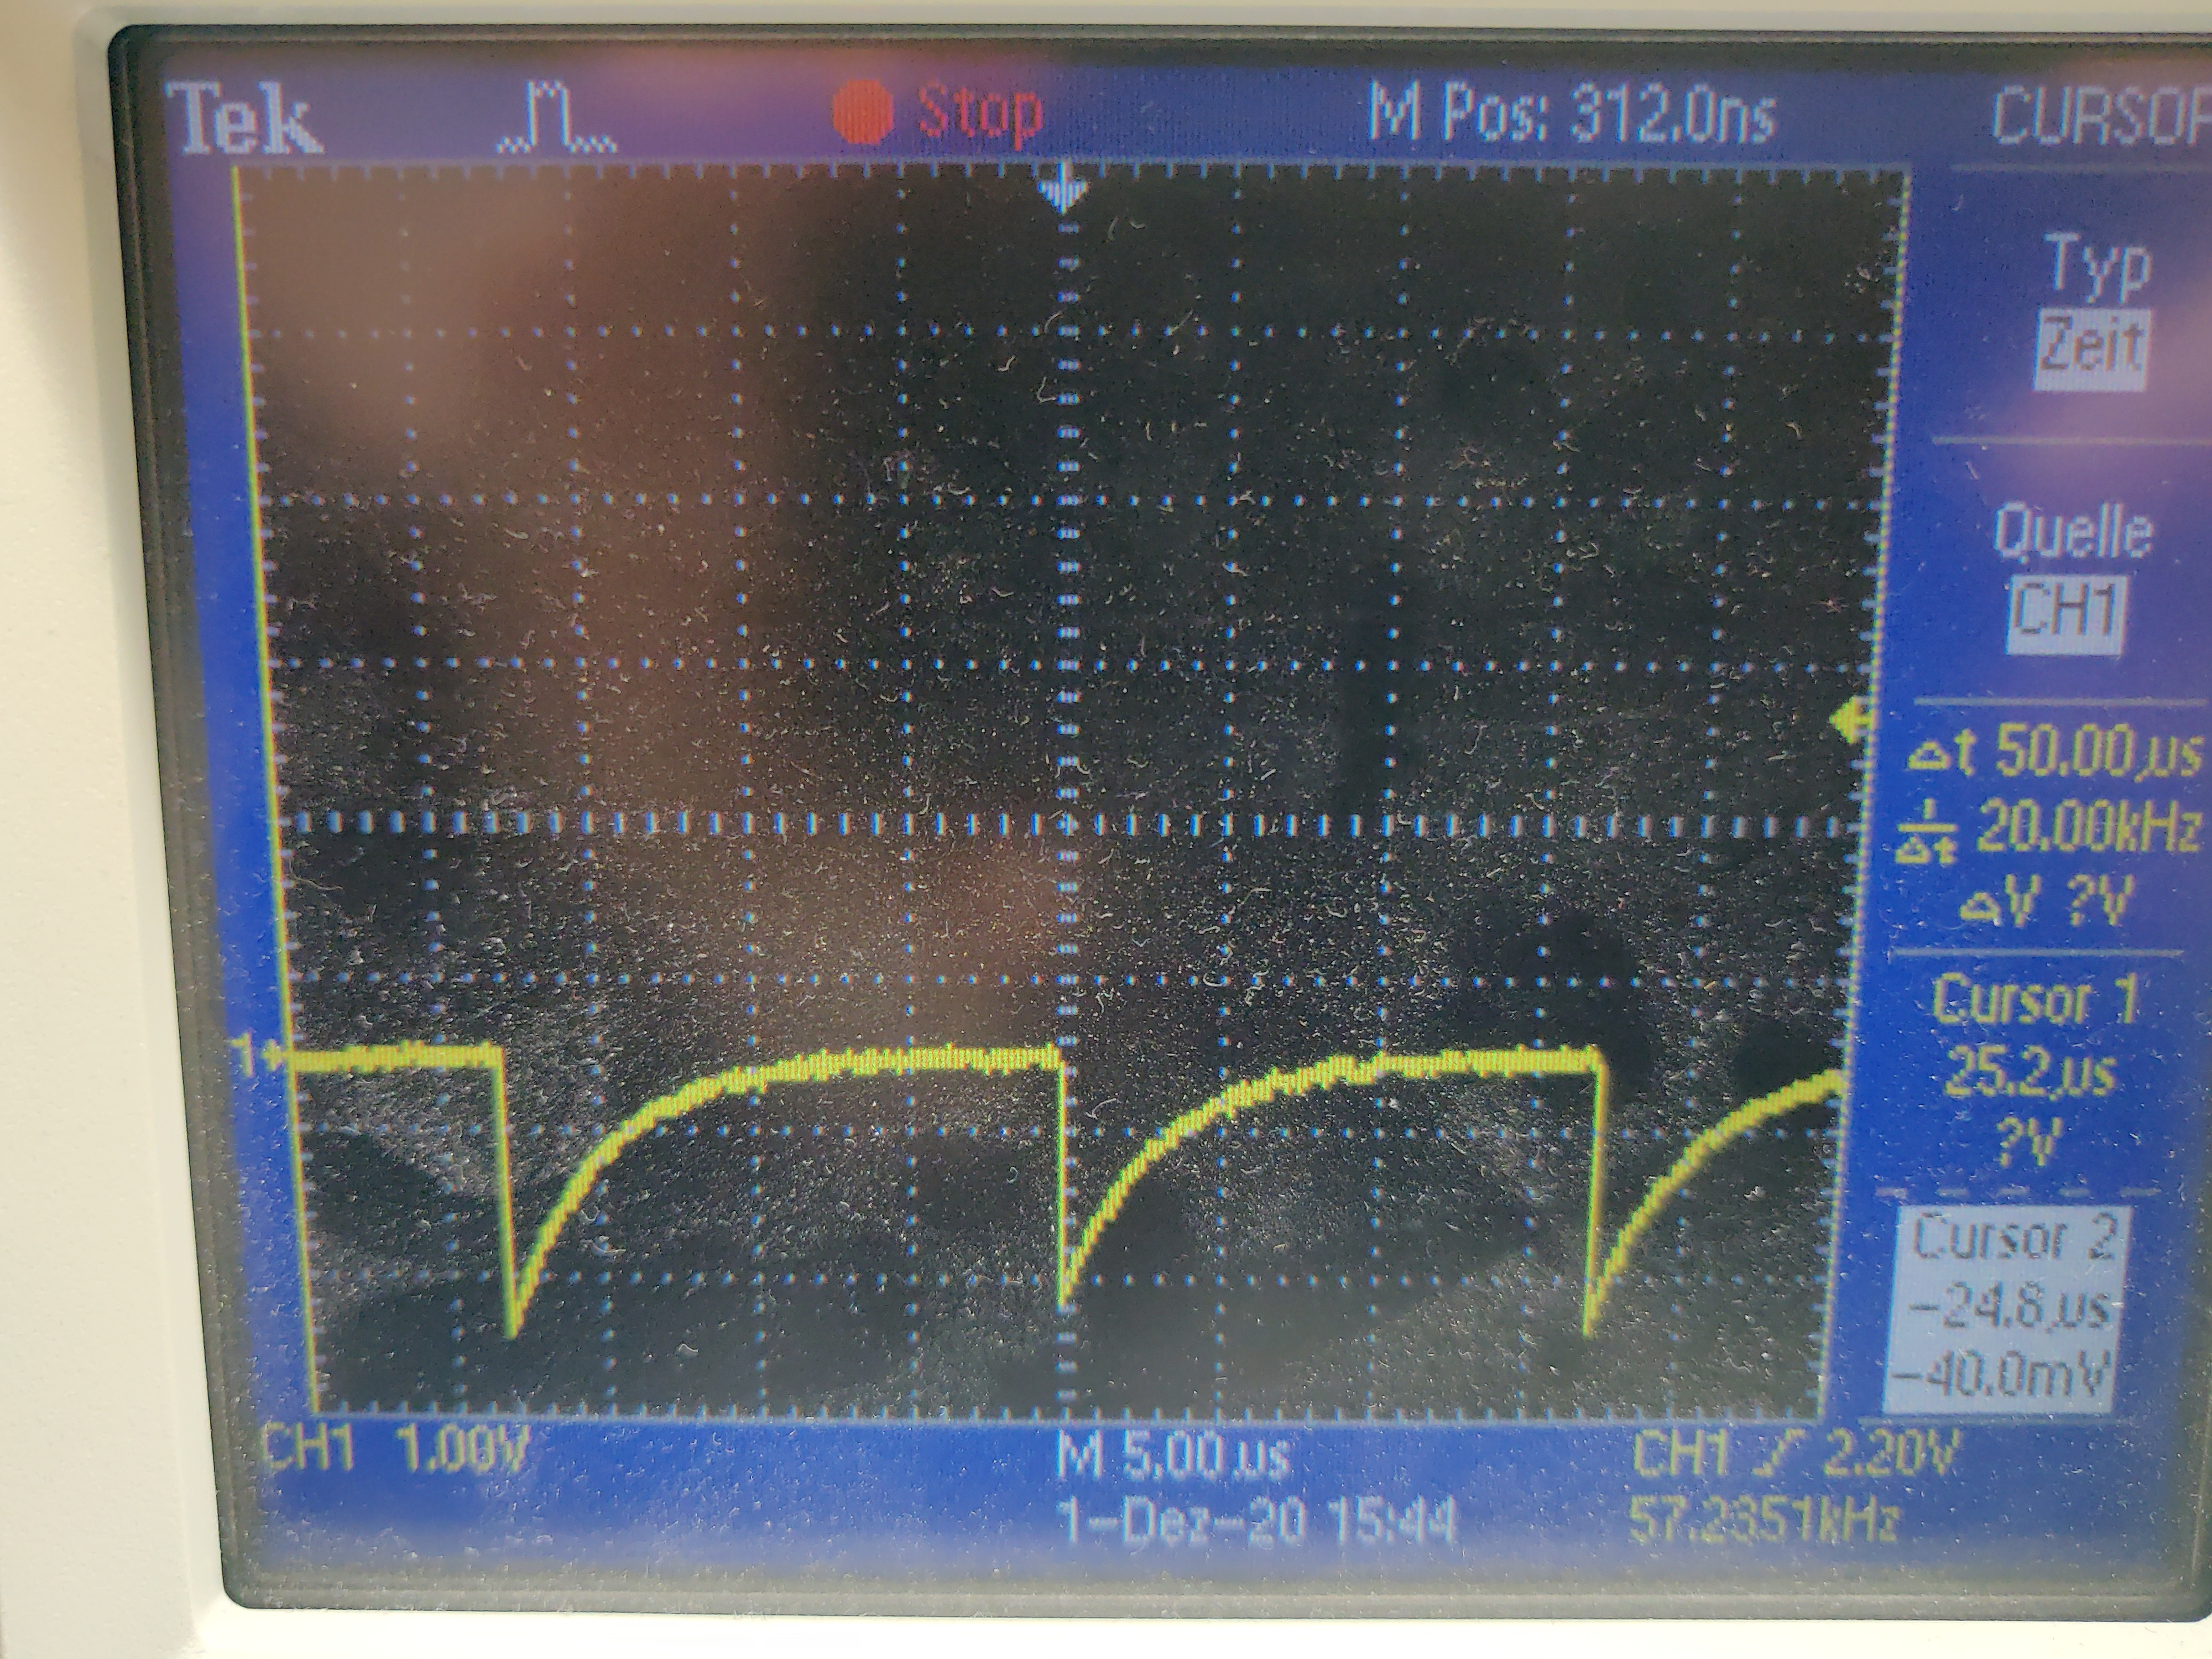
\includegraphics[width=0.7\linewidth]{messdaten/IMG_20201201_084956}
 \caption[Avalanche pulse signal at $ U_{min} $]{Avalanche pulse signal at $ U_{min} $}
 \label{fig:img20201201084956}
\end{figure}
The repetition frequency of the avalanche pulse generator has been investigated and recorded as shown in \vref{fig:repetition-frequency}.
\begin{figure}[H]
 \centering
 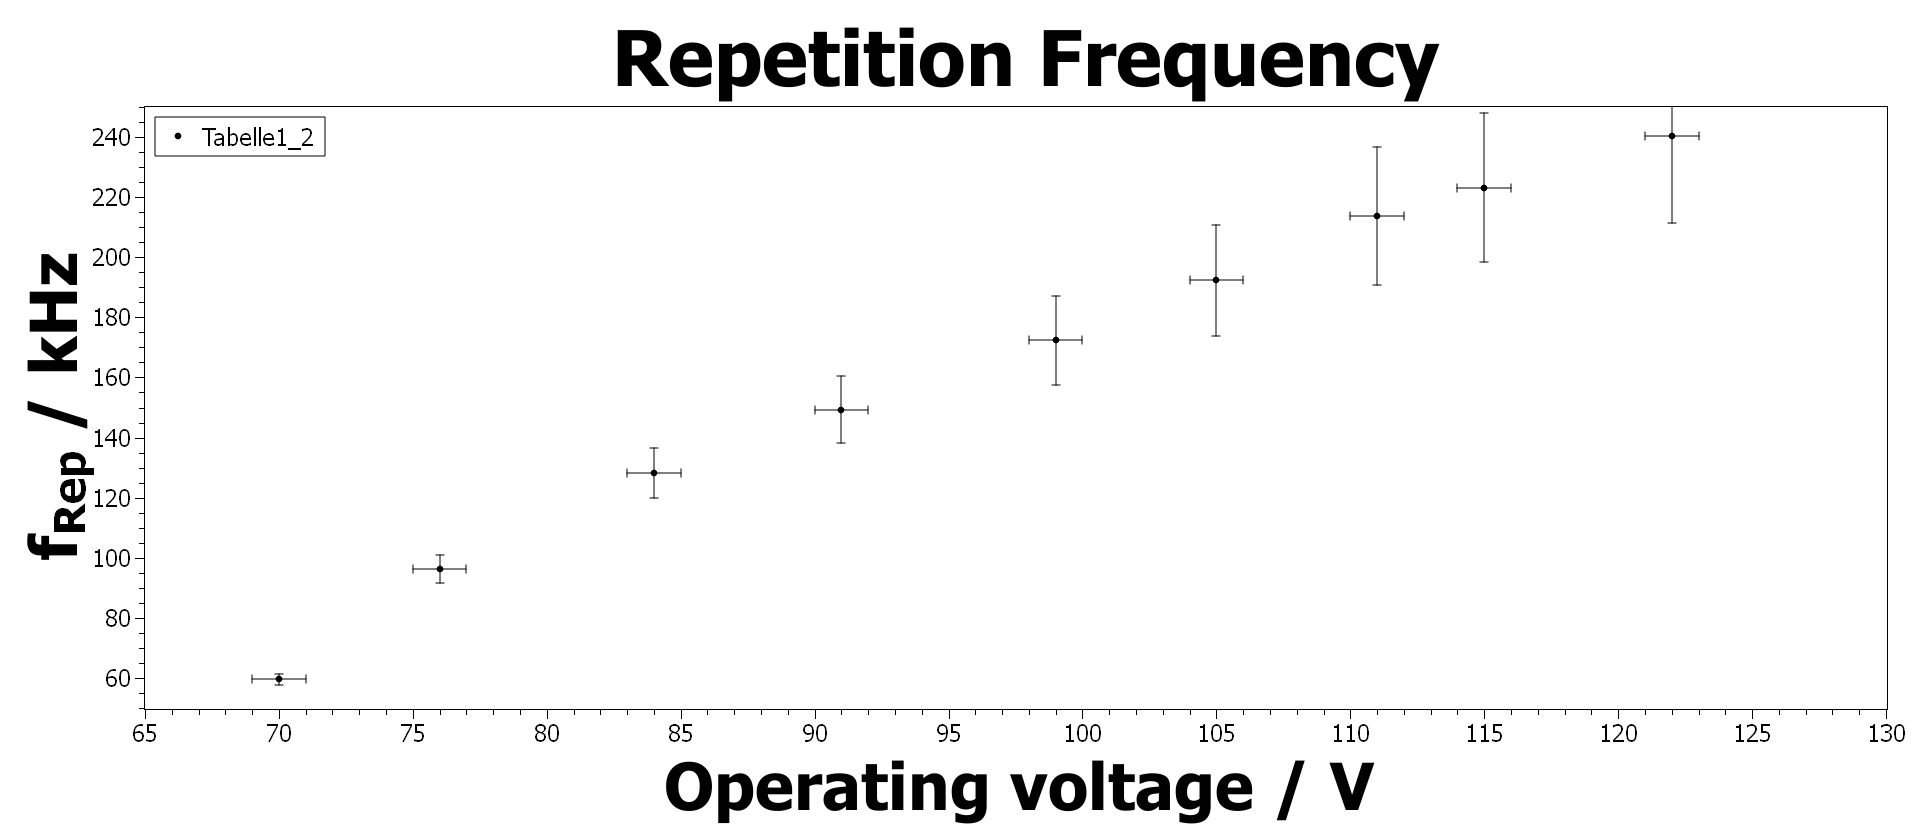
\includegraphics[width=1\linewidth]{messdaten/Repetition Frequency}
 \caption[Repetition frequency]{Repetition frequency}
 \label{fig:repetition-frequency}
\end{figure}
In section 2.2 the theoretical value for the repetition frequency at $ U=\SI{75}{V} $ was calculated as $ f_{Rep}=\SI{225.7}{kHz} $. In the diagram in \vref{fig:repetition-frequency} the value is around $ \SI{90}{kHz} $. So there must be some deviations.\\\\
Next the characteristics of the pulse at a voltage of $ U=\SI{75}{V} $ are examined. Fig. \ref{fig:pulsuntersuchung} gives the following:
\begin{align}
\text{Amplitude:}\qquad Û&=\SI{7.12}{V}\\
\text{Rise time:}\qquad t_r&=\SI{2.33}{s}\\
\text{Fall time:}\qquad t_f&=\SI{7.08}{s}\\
\text{Pulse width:}\qquad t_w&=\SI{6.26}{s}
\end{align}
\begin{figure}[H]
 \centering
 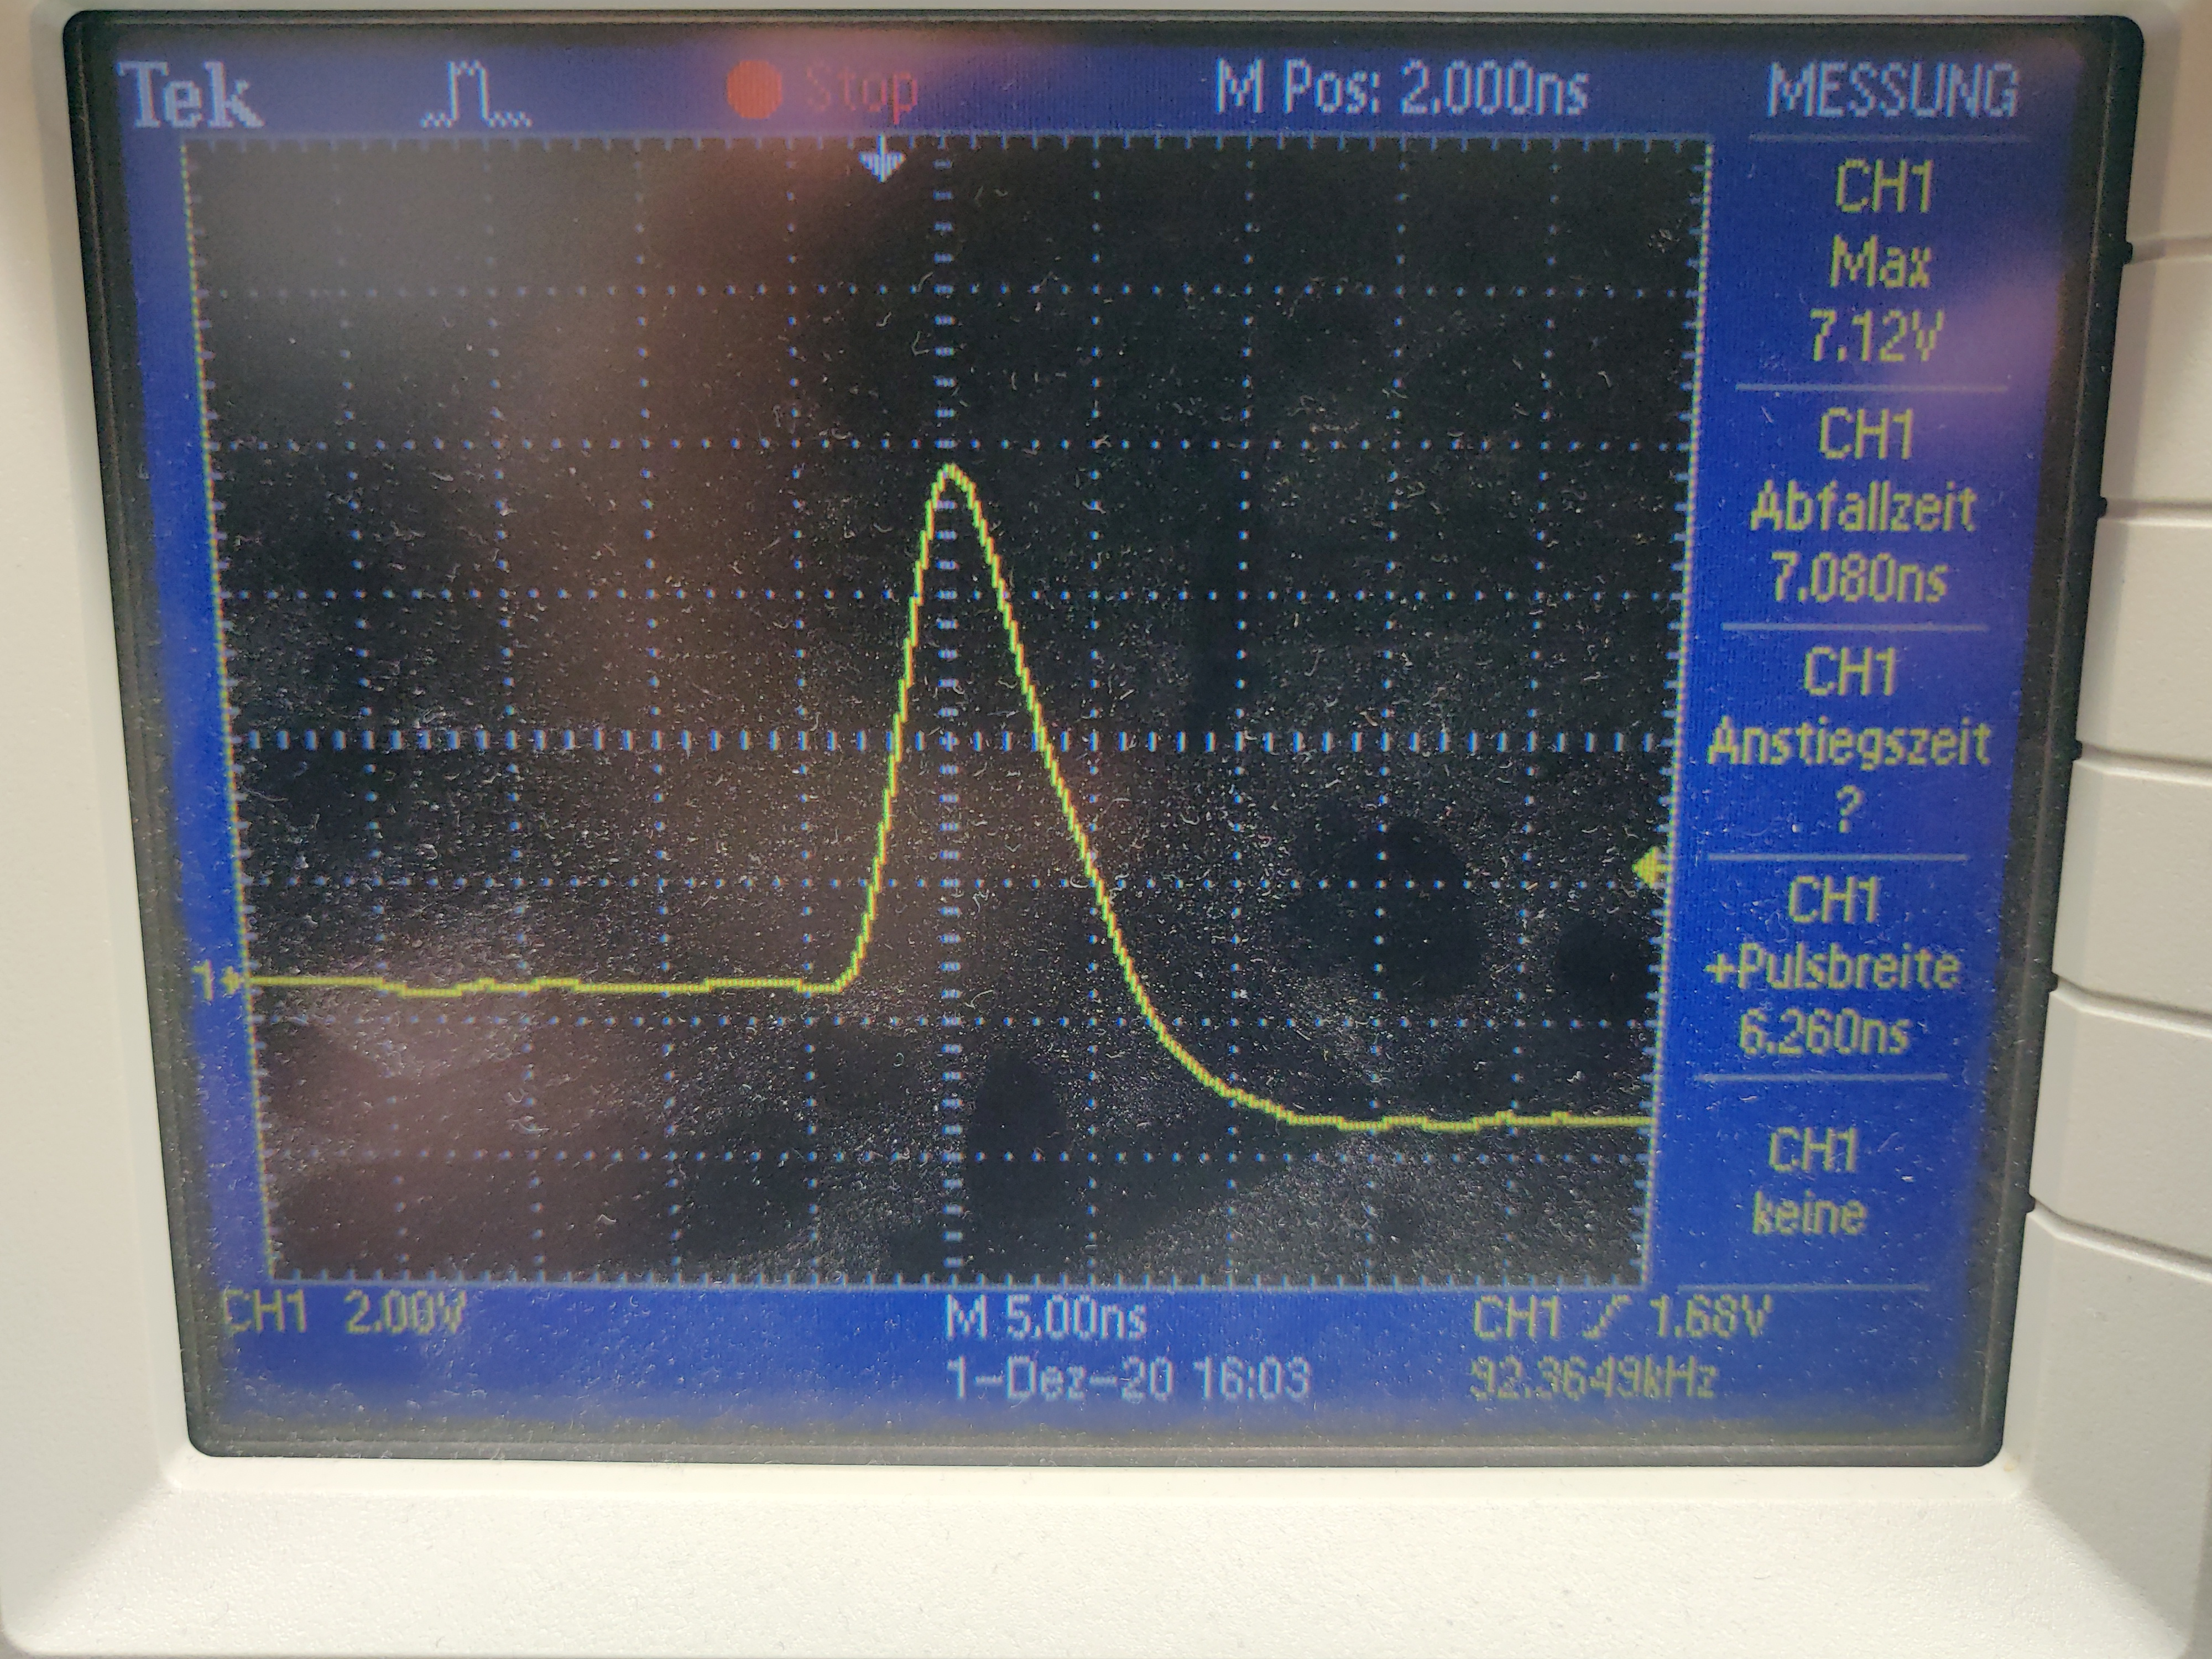
\includegraphics[width=0.7\linewidth]{messdaten/Pulsuntersuchung}
 \caption[Pulse characteristics]{Pulse characteristics}
 \label{fig:pulsuntersuchung}
\end{figure}
In comparison to a 500 MHz oscilloscope signal, it can be seen that the secondary pulsations are drawn more accurate in the 500 MHz oscilloscope. Rise and fall time and the pulse width is much shorter. Even the amplitude seems to be larger. Reason for this could be the higher capacity due to the higher bandwidth for more precise and better approximations.

\section{Signal Propagation}

\subsection{Propagation Time}
The propagation speed can be determined by means of:
\begin{equation}
c_P=\frac{l}{t}
\end{equation}
The measured propagation times and the calculated propagation speeds are summarized in the following table:
\begin{table}[H]
 \caption{Delayed signal}
 \centering
 \begin{tabular}{|c|c|c|c|}
 \hline 
 Cable no. & $ l \pm \Delta l $ \big/ \SI{}{m} & $ t \pm \Delta t $ \big/ \SI{}{ns} & $ c_P \pm \Delta c_P $ \big/ $ \SI{}{\frac{m}{s}} $ \\ 
 \hline 
 \hline
 1 & $ 4.95 \pm 0.05 $ & $ 22.6 \pm 1 $ & $ (2.19\pm 0.12)\cdot 10^8 $ \\ 
 \hline 
 2 & $ 10.04 \pm 0.05 $ & $ 44.8 \pm 1 $ & $ (2.24\pm 0.06)\cdot 10^8  $ \\ 
 \hline 
 3 & $ 0.77 \pm 0.01 $ & $ 4.6 \pm 1 $ & $ (1.67\pm 0.39)\cdot 10^8 $ \\ 
 \hline 
\end{tabular}
\label{delayed signal}
\end{table}
The deviation of the propagation speed can be determined as follows:
\begin{align}
\Delta c_P&=\left|\frac{\partial c_P}{\partial l}\right|\cdot \Delta l + \left|\frac{\partial c_P}{\partial t}\right|\cdot \Delta t\\
&=\frac{1}{t}\cdot \Delta l + \frac{l}{t^2} \cdot \Delta t \label{cp dev}
\end{align}
For cable no. 1 in \vref{delayed signal} e.g.:
\begin{align*}
\Delta c_{P,1}&=\frac{1}{\SI{22.6}{\cdot 10^{-9}s}}\cdot \SI{0.05}{m} + \frac{\SI{4.95}{m}}{(\SI{22.6}{\cdot 10^{-9}s})^2} \cdot \SI{1}{\cdot 10^{-9}s}\\
&=\SI{0.02}{\cdot 10^8\frac{m}{s}}+\SI{0.10}{\cdot 10 ^8\frac{m}{s}}\\
&=\SI{0.12}{\cdot 10^8\frac{m}{s}}
\end{align*}

\subsection{Cable Characteristics}
Fig.\ref{fig:3-3-2reflectiontime} shows the reflected pulse signal and \vref{fig:3-3-2shorted} the shorted and reflected pulse signal.
\begin{figure}[p]
 \centering
 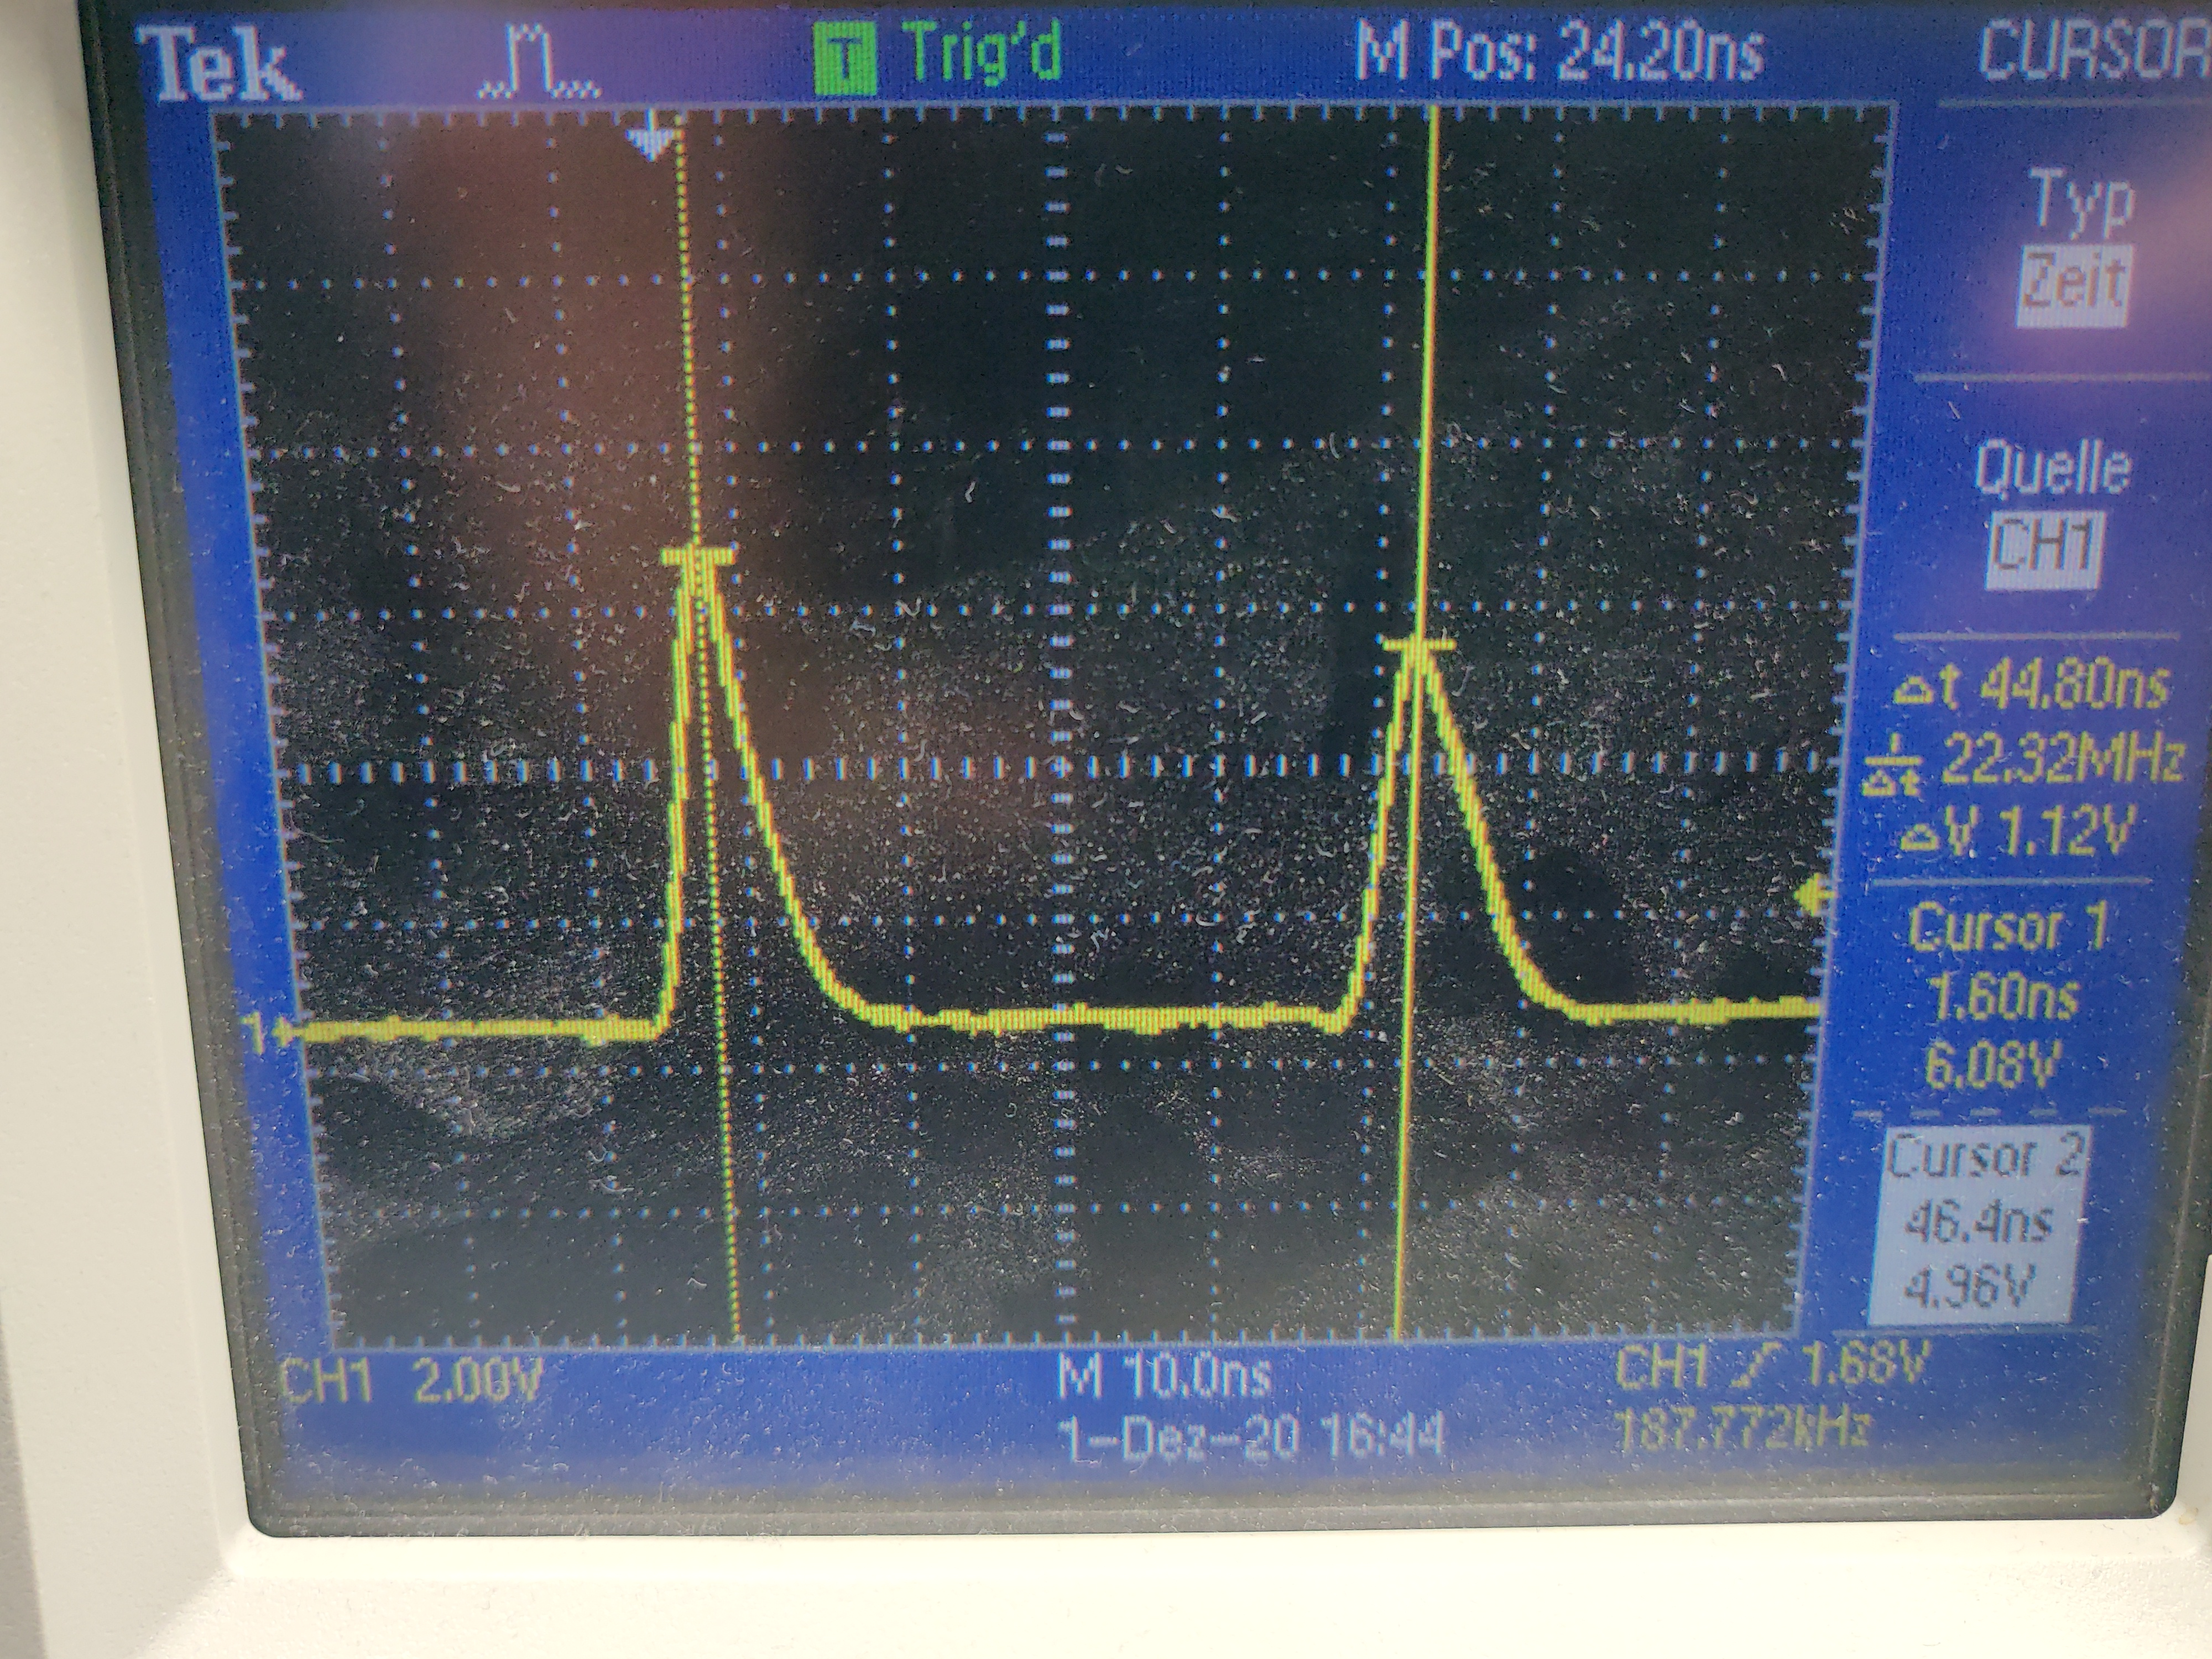
\includegraphics[width=0.7\linewidth]{messdaten/3-3-2_reflectionTime}
 \caption[Reflected pulse signal]{Reflected pulse signal}
 \label{fig:3-3-2reflectiontime}
\end{figure}
\begin{figure}[p]
 \centering
 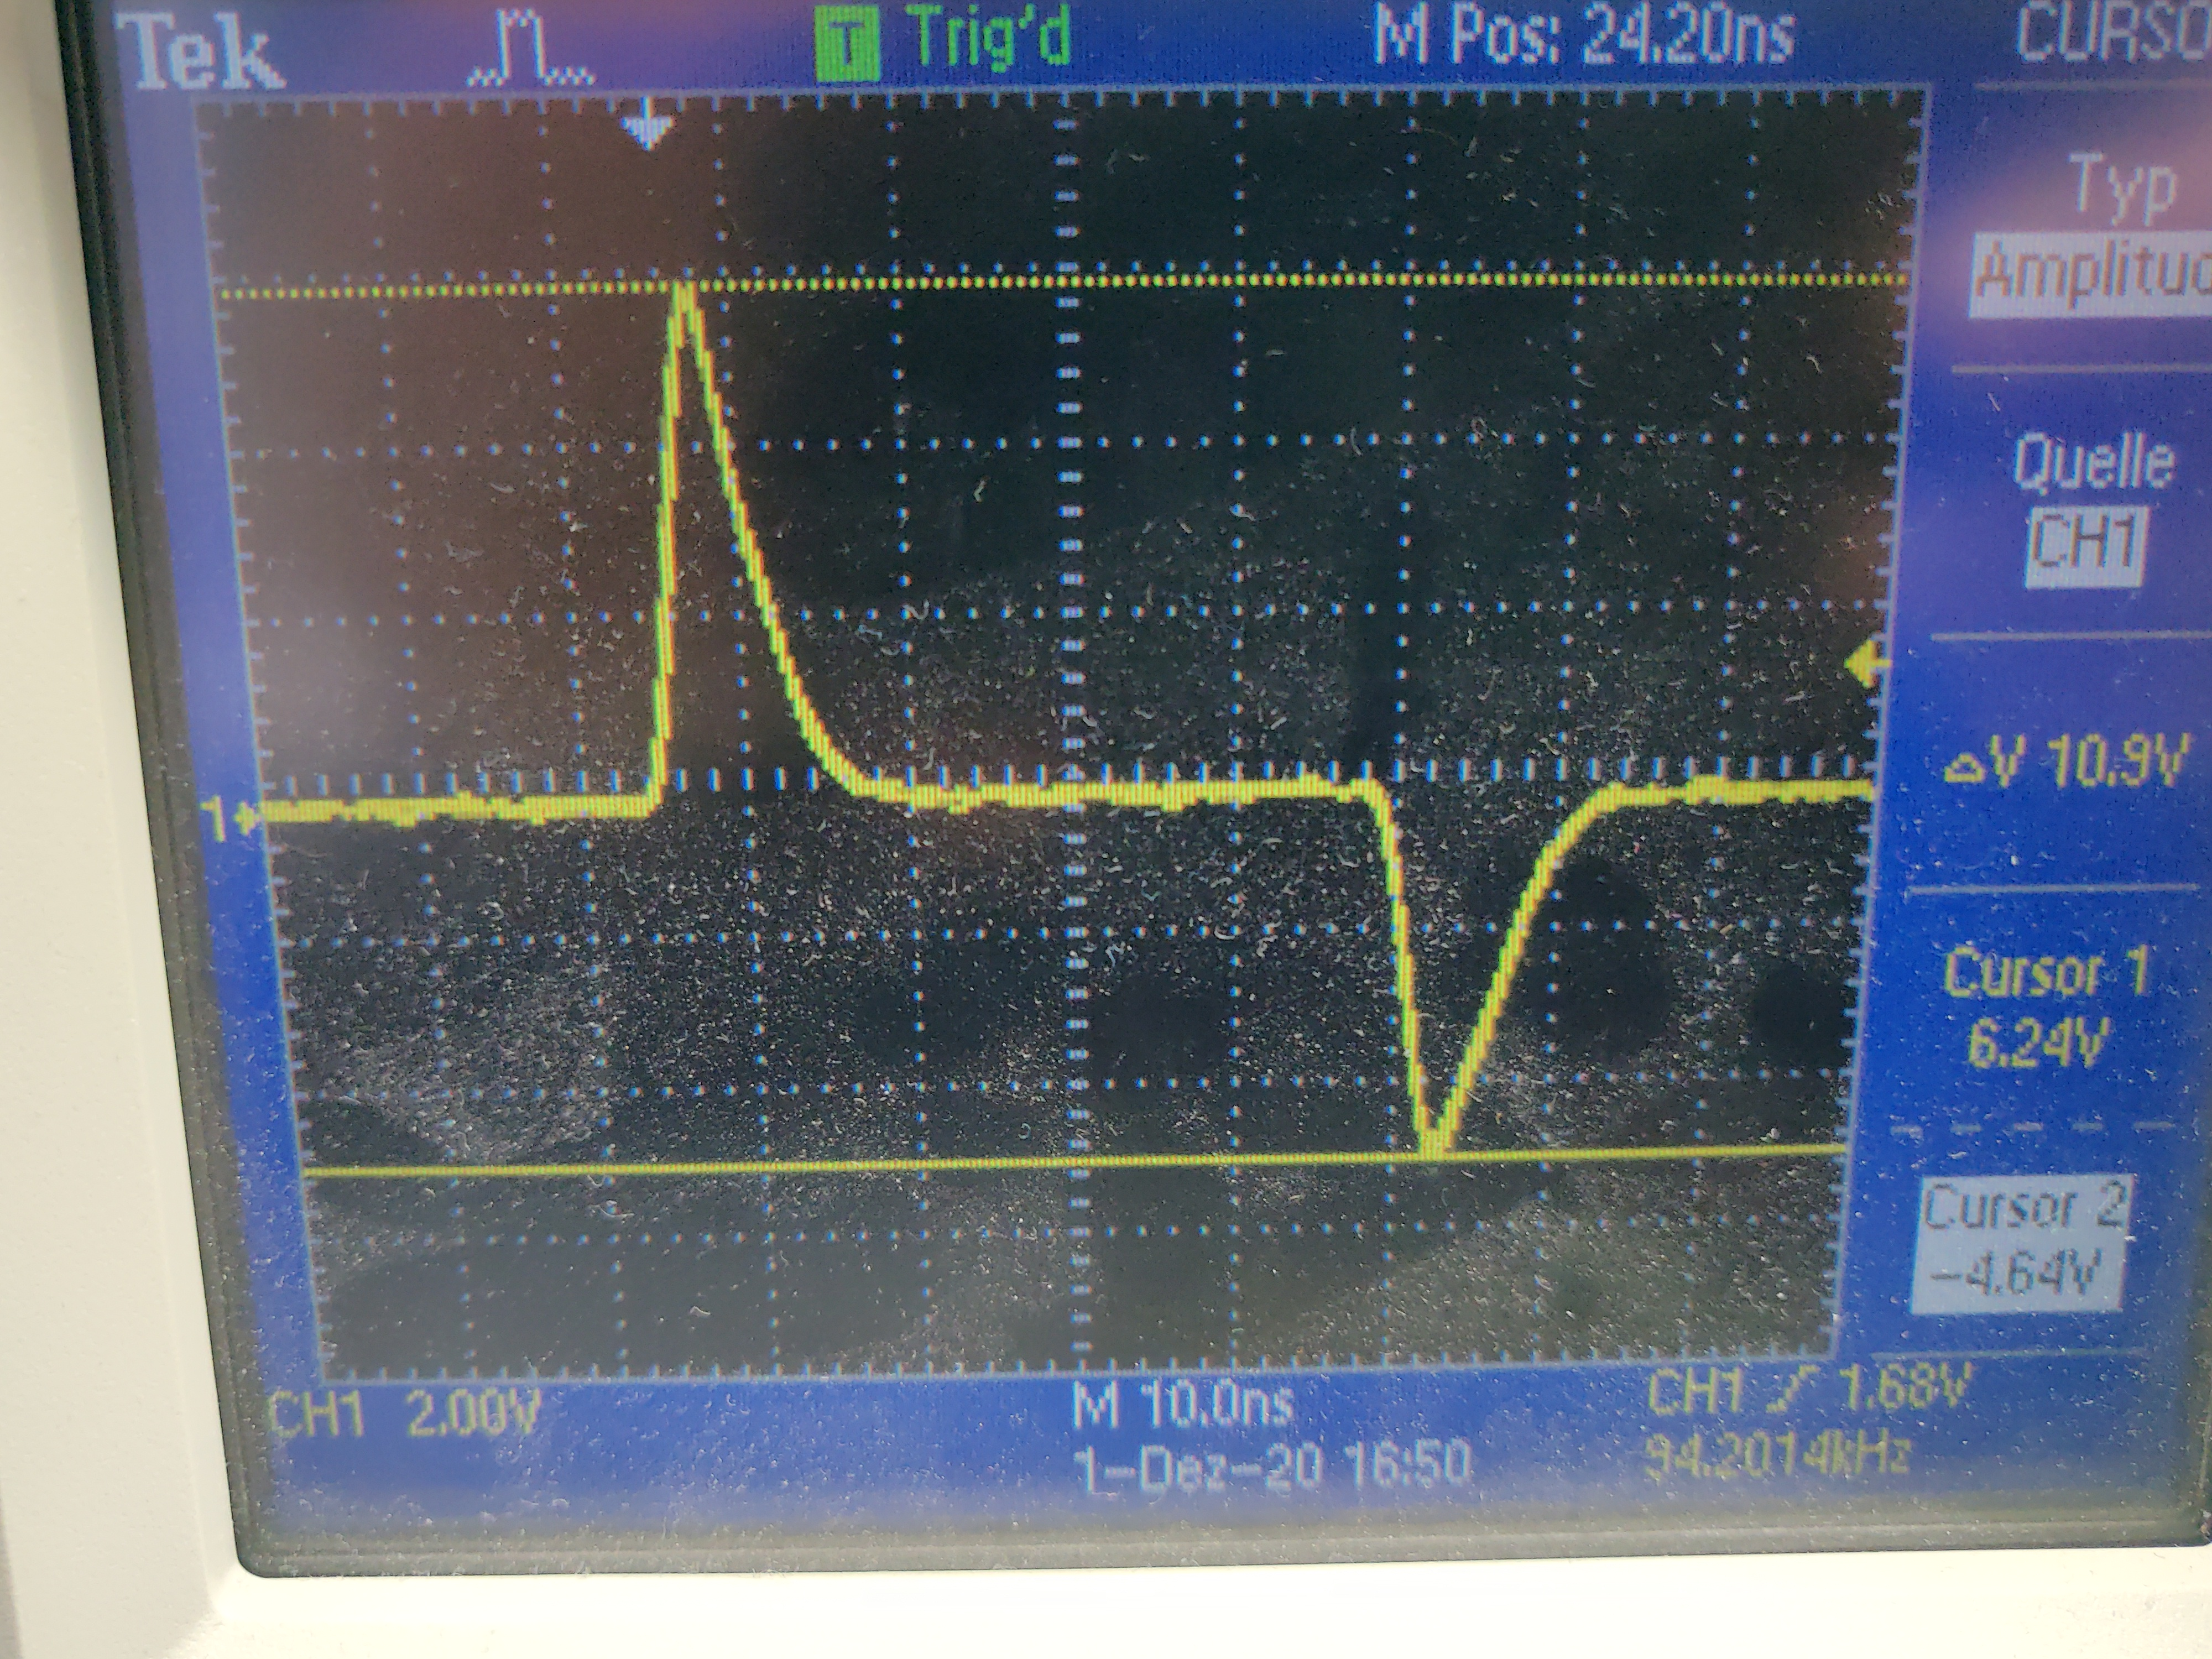
\includegraphics[width=0.7\linewidth]{messdaten/3-3-2_shorted}
 \caption[Shorted pulse signal]{Shorted pulse signal}
 \label{fig:3-3-2shorted}
\end{figure}
The propagation speed can be calculated with eq.(6), the velocity factor with eq.(7) and the relative dielectric constant with eq.(9) of the instructions. At the minimum amplitude of the reflected pulse, the resistance $ R_{Term} $ equals $ Z_0 $.\\
The determined and calculated characteristic values are summarized in the following table:
\begin{table}[H]
 \caption{Reflected signal}
 \begin{tabular}{|c|c|c|c|c|c|c|c|}
  \hline 
  Cable no. & $ l $ \big/ \SI{}{m} & $ \tau_0 $ \big/ \SI{}{ns} & $ \tau_s $ \big/ \SI{}{ns} & $ c_P $ \big/ $ \SI{}{\frac{m}{s}} $ & $ VF $ \big/ \% & $ Z_0 $ \big/ $\Omega$ & $\varepsilon_R$ \\ 
  \hline 
  \hline
  1 & $ 4.95 \pm 0.05 $ & $ 44.8 \pm 1 $ & $ 44.8 \pm 1 $ & $ (2.21\pm 0.07)\cdot 10^8 $ & $ 73.7 \pm 2.3 $ & 80.2 & $ 1.84 \pm 0.11 $ \\ 
  \hline 
  2 & $ 10.04 \pm 0.05 $ & $ 89.6 \pm 1 $ & $ 90.4 \pm 1 $ & $ (2.24\pm 0.04)\cdot 10^8 $ & $ 74.7 \pm 1.3 $ & 56.0 & $ 1.79 \pm 0.06 $ \\ 
  \hline 
  3 & $ 0.77 \pm 0.01 $ & $ 8.4 \pm 1 $ & $ 10.8 \pm 1 $ & $ (1.83\pm 0.34)\cdot 10^8 $ & $ 61.0 \pm 11.3 $ & 56.4 & $ 2.69 \pm 1.00 $ \\ 
  \hline 
 \end{tabular}
 \label{reflected signal}
\end{table}
The deviation of $ c_P $ can be determined similar to \vref{cp dev}, but with a factor of 2. The one of $ VF $ as follows:
\begin{align}
\Delta VF&=\left|\frac{\partial VF}{\partial c_P}\right|\cdot \Delta c_P\\
&=\frac{1}{c_0}\cdot \Delta c_P
\end{align}
For cable no. 1 in \vref{reflected signal} e.g.:
\begin{equation*}
\Delta VF_1=\frac{1}{\SI{3}{\cdot 10^8 \frac{m}{s}}}\cdot \SI{0.07}{\frac{m}{s}}=2.3\%
\end{equation*}
And for $ \varepsilon_R $:
\begin{align}
\Delta \varepsilon_R&=\left|\frac{\partial \varepsilon_R}{\partial VF}\right|\cdot \Delta VF\\
&=\frac{2}{VF^3}\cdot \Delta VF
\end{align}
So for the first cable in \vref{reflected signal}:
\begin{equation*}
\Delta \varepsilon_{R,1}=\frac{2}{0.737^3}\cdot 0.023=0.11
\end{equation*}
If the values are compared with the data sheet from the manufacturer, there can be seen some similarities and differences. The determined velocity factor of cable no. 1 and 2 is very close to the stated one (69.5\%). The third cable is slightly different.
On the other hand, the impedance is given as $ \SI{53}{\Omega} $, with the second and third cable having a similar value, whereas the first cable differs somewhat.

\subsection{Time Domain Reflectometry}
For determining the unknown length and the position of the fault of the cable, the equation for the propagation speed has to be transformed to the length as
\begin{equation}
l=\frac{1}{2}\cdot c_P \cdot \tau
\label{length}
\end{equation}
$\tau_{total}$ has been measured as $ \tau_{total}=\SI{276}{ns} $ and $\tau_{fault}$ as $ \tau_{fault}=\SI{256}{ns} $.
For the propagation speed the mean value $ \bar{c_P}=\SI{2.09}{\cdot 10^8\frac{m}{s}} $ is used. The values inserted in \vref{length} results:
\begin{align*}
l_{total}&=\frac{1}{2}\cdot\SI{2.09}{\cdot 10^8\frac{m}{s}}\cdot \SI{276}{\cdot 10^{-9} s}=\SI{28.84}{m}\\
l_{fault}&=\frac{1}{2}\cdot\SI{2.09}{\cdot 10^8\frac{m}{s}}\cdot \SI{256}{\cdot 10^{-9} s}=\SI{26.75}{m}
\end{align*}
The deviation is determined with the following equation:
\begin{align}
\Delta l&=\left|\frac{\partial l}{\partial c_P}\right|\cdot \Delta c_P + \left|\frac{\partial l}{\partial \tau}\right|\cdot \Delta \tau\\
&=\frac{1}{2}\cdot \tau \cdot \Delta c_P + \frac{1}{2}\cdot c_P \cdot \Delta \tau
\end{align}
For the total length and the faultposition:
\begin{align*}
\Delta l_{total}&=\frac{1}{2} \cdot\SI{276}{\cdot 10^{-9}s}\cdot \SI{0.15}{\cdot 10^8\frac{m}{s}}  + \frac{1}{2}\cdot \SI{2.09}{\cdot 10^8\frac{m}{s}} \cdot\SI{1}{\cdot 10^{-9}s}\\
&=\SI{2.07}{m}+\SI{0.10}{m}\\
&=\SI{2.17}{m}\\
\\
\Delta l_{fault}&=\SI{2.02}{m}
\end{align*}
Summarized the total length is
\begin{equation}
l_{total}=\SI{28.8}{m} \pm \SI{2.2}{m}
\end{equation}
and the position of the fault is at
\begin{equation}
l_{fault}=\SI{26.8}{m} \pm \SI{2.0}{m}
\end{equation}